%%%%%%%%%%%%%%%%%%%%%%%%%%%%%%%%%%%%%%%%%%%%%%%%%%%%%%%%%%%%%%%
%
% Introduction.tex (part of thesis.tex)
% author: Qie Hu
%
%%%%%%%%%%%%%%%%%%%%%%%%%%%%%%%%%%%%%%%%%%%%%%%%%%%%%%%%%%%%%%%

%!TEX root = ../../thesis.tex

\subsection{Model Identification}\label{sec:model_id}

\subsubsection{Building Model}\label{sec:building_model}

In \cite{Zhou:2017modelcomp}, we proposed a semiparametric method for identifying a data-driven linear and low-dimensional building model.
Extensive quantitative comparison between this model and a physics-based nonlinear and high-dimensional model was carried out using experimental data, and we concluded that the data-driven model is suitable for applications such as frequency regulation due to its minor loss of prediction accuracy, but significant gain in computational ease.
Consequently, the data-driven model is used in this work. 
In the rest of this section, we summarize this identification method.

%Traditionally, VAV HVAC systems of commercial buildings have been modeled with bilinear high-dimensional physics-based models, which are computationally expensive and not amenable to control.
%In our previous work \cite{Zhou:2017modelcomp}, we identified both a linear low-dimensional data-driven model and a bilinear high-dimensional physics-based model for the fourth floor of SDH, and made extensive quantitative comparison of both models using experimental data.
%We concluded that the low-dimensional data-driven model is suitable for applications such as frequency regulation due to its minor loss of prediction accuracy, but significant gain in computational ease.
%Consequently, we identify 

%Traditionally, buildings have been modeled with high-dimensional physics-based models. Furthermore, such models are bilinear in nature if the buildings are equipped with VAV HVAC systems \cite{Qie}. The high-dimensionality and bilinearity make them computationally difficult.
%In \cite{Zhou_modelcomp}, the authors identified both a linear low-dimensional data-driven model and a bilinear high-dimensional physics-based model for the fourth floor of SDH. Extensive quantitative comparison of both models were conducted in terms of open-loop prediction accuracy and closed-loop control strategies, using experimental data collected from the building.
%They concluded that the low-dimensional data-driven model is suitable for building control applications, such as frequency regulation, due to its minor loss of prediction accuracy compared to the high dimensional physics-based model, but significant gain in computational ease.
%Consequently, we use the data-driven model identified in \cite{Zhou_modelcomp} in our experiments.
%In the rest of this section, we briefly describe the identification of this input-output model. 

%%%%%%%%%%%%%%%%%%%%%%%%%%%%%%%%%%%%%%%%%%%%%%
%%%%%%%%%%%%%%%%%%%%%%%%%%%%%%%%%%%%%%%%%%%%%%

\subsubsection{Collection of Experimental Data}\label{sec:building_model_data}

We collected 51 weeks of one-minute resolution temperature data for the six zones along with the airflow rates of the VAV boxes, SAT and the outside air temperature from the \textit{simple Measurement and Actuation Profile} (sMAP), which is a protocol that collects, stores and publishes time-series data from a wide variety of sensors \cite{smap, Dawson-Haggerty:2012aa}. 

These 51 weeks of data span periods when the building was under normal operation as well as periods with excitation experiments. To increase identifiability of the building model, forced response experiments were performed. These experiments were conducted during Saturdays to (a) minimize effects due to occupancy on our collected data, and thus facilitate subsequent parameter identification; (b) minimize impact to building operation and exploit larger comfort bounds on room temperatures during the weekends. Indeed, the comfort bounds were never violated during the forced experiments. Details on the design of our excitation experiments can be found in \cite{Qie}.

A random portion of the 51 weeks of data (e.g. we chose 90\%) was defined as the training data, and the remaining weeks were removed prior to the analysis and declared as the test set.

%%%%%%%%%%%%%%%%%%%%%%%%%%%%%%%%%%%%%%%%%%%%%%
%%%%%%%%%%%%%%%%%%%%%%%%%%%%%%%%%%%%%%%%%%%%%%

%\subsubsection{Data Splitting}
%Next, we defined the seasons ``fall" (early September until mid December), ``winter" (mid December until late January), and ``spring" (late January until mid May) in order to account for different occupancy levels during the fall and spring semesters, and the winter break. After the weeks have been assigned to the seasons, a random portion of the data in each season (e.g. we chose 90\%) was defined as the training data, and the remaining weeks to be removed prior to the analysis were declared as the test set, which were used to assess the accuracy of the building model fitted on the training data.

%%%%%%%%%%%%%%%%%%%%%%%%%%%%%%%%%%%%%%%%%%%%%%
%%%%%%%%%%%%%%%%%%%%%%%%%%%%%%%%%%%%%%%%%%%%%%

\subsubsection{Model Setup}

Define the vector $x \in \mathbb{R}^6$ as the average temperature in each of the six zones (see Figure \ref{fig:floor_plan}) and the input vector $u \in \mathbb{R}^6$ as the total airflow to each zone. Then, the temperature evolution is assumed to have the following form:

\begin{equation}
\begin{aligned}\label{eq:building_model}
x_{k+1} &= A x_k + B u_k + C v_k + q_k + \epsilon_k, \\
\end{aligned}
\end{equation}
%\begin{equation}
%\begin{aligned}\label{eq:building_model_indiv}
%x(k+1) &= A x(k) + B u(k) + C v(k) + q_{\text{IG},\mathcal{X}}(k) \\
%& ~~ \text{for } \mathcal{X} \in \lbrace \mathcal{F}, \mathcal{W}, \mathcal{S} \rbrace,
%\end{aligned}
%\end{equation}
where $v:= \left[ v_\text{Ta}, v_\text{Ts} \right]^\top \in \mathbb{R}^2$ is a disturbance vector that describes ambient air temperature and the HVAC system's SAT\footnote{It was found in \cite{Zhou:2017modelcomp} that solar radiation had a negligible effect on the indoor temperatures on the fourth floor, therefore it is not included in this model.}, and  $q \in \mathbb{R}^6$ represents the internal gains due to occupancy and electric devices.
$\epsilon$ denotes independent and identically distributed zero mean noise with constant and finite variance which is conditionally independent of $x$, $u$, $v$, and $q$. Finally, $A$, $B \in \mathbb{R}^{6\times6}$ and $C \in \mathbb{R}^{6\times2}$ are unknown coefficient matrices to be estimated using semiparametric regression \cite{Ruppert:2003aa, Hardle:2000aa}.

%%%%%%%%%%%%%%%%%%%%%%%%%%%%%%%%%%%%%%%%%%%%%%
%%%%%%%%%%%%%%%%%%%%%%%%%%%%%%%%%%%%%%%%%%%%%%

\subsubsection{Smoothing of Time Series}

The $q$ term of Equation \eqref{eq:building_model} is treated as a nonparametric term, so that \eqref{eq:building_model} becomes a partially linear model. By taking conditional expectations on both sides of \eqref{eq:building_model}, we obtain
\begin{equation}\label{eq:Conditional_Expectation}
\hat{x}_k = A\hat{x}_k + B\hat{u}_k + C\hat{v}_k + \mathbb{E}\left[ q_k \vert k \right] + \mathbb{E}\left[ \epsilon_k \vert k \right],
\end{equation}
\noindent
where the conditional expectations $\hat{x}_k = \mathbb{E}\left[ x_k \vert k \right]$, $\hat{u}_k = \mathbb{E}\left[ u_k \vert k \right]$, and $\hat{v}_k = \mathbb{E}\left[ v_k \vert k \right]$ are used.
Noting that $\mathbb{E}\left[ \epsilon_k \vert k \right] = 0$ for all $k$ and assuming $\mathbb{E}\left[ q_k \vert k \right] = q_k$ for all $k$, subtracting \eqref{eq:Conditional_Expectation} from \eqref{eq:building_model} gives
\begin{equation}\label{eq:subtract}
\begin{split}
x_{k+1} - \hat{x}_{k+1} = A\left( x_k - \hat{x}_k \right) + B\left( u_k - \hat{u}_k \right) \\
+ C \left( v_k - \hat{v}_k \right) + \epsilon_k.
\end{split}
\end{equation}
The unknown internal gains term has been eliminated, and thus the coefficient matrices $A$, $B$ and $C$ in \eqref{eq:subtract} can be estimated with any regression method.
The conditional expectations $\hat{x}_k, ~\hat{u}_k$ and $\hat{v}_k$ are obtained by smoothing the respective time series \cite{Aswani:2012aa}. 
%We made use of locally weighted linear regression with a tricube weight function, where we use $k$-fold cross-validation to determine the bandwidth for regression.

%The error measure used for in-sample estimates is the \textit{Root Mean Squared} (RMS) \textit{Error} between the measured temperatures $\bar{x}(k)$ and the model's predicted temperatures $x(k)$ over a time horizon of $N$ steps (e.g. we chose a 24 hour time horizon, $N = 96$):
%\begin{equation}\label{eq:RMS}
%\text{RMS error} = \left(\frac{1}{N}\textstyle\sum_{k=1}^N \left[\bar{x}(k) - x(k)\right]^2 \right)^{1/2}.
%\end{equation}

%%%%%%%%%%%%%%%%%%%%%%%%%%%%%%%%%%%%%%%%%%%%%%
%%%%%%%%%%%%%%%%%%%%%%%%%%%%%%%%%%%%%%%%%%%%%%

\subsubsection{Bayesian Constrained Least Squares}

To overcome the challenge of insufficient excitation of the building, data collected during forced response experiments is used in training the model. Furthermore, 
%A main challenge in identifying the model is that commercial buildings are often insufficiently excited. Take SDH for example, whose room temperatures under regular operation only vary within a range of 2$^{\circ}$C and inflow of the VAV boxes hardly varies at all. To overcome this, 
a Bayesian regression method is used, which allows our prior knowledge of the building physics to be incorporated in the identification of coefficients. 
In particular, Gaussian prior distributions are used for the coefficient matrices $A$, $B$ and $C$, i.e., $vec(A) \sim \mathcal{N}( \mu_A, \Sigma_A)$, $vec(B) \sim \mathcal{N}( \mu_B, \Sigma_B)$, and $vec(C) \sim \mathcal{N}( \mu_C, \Sigma_C)$ where $vec(M)$ represents the vectorized form of matrix $M$ and $\mathcal{N}( \mu, \Sigma)$ denotes a jointly Gaussian distribution with mean $\mu$ and covariance matrix $\Sigma$. 
%In addition, $a$, $b$ and $c$ are constrained to be identical for the different seasons, since they model the underlying physics of the building which are assumed to be invariant throughout the year. 
The mean vectors and covariance matrices were chosen subjectively and the sparsity pattern of the coefficient matrices $A$, $B$ and $C$ are defined by physics such as adjacency of the zones to each other and to exterior walls.

%In addition, inspired by Newton's Law of Cooling, only adjacent zones influence each other's temperature, which defines the sparsity pattern of the coefficient matrices that are to be estimated. Hence 
%\begin{equation}
%A_{ij} = \begin{cases}
%      \neq 0, & \text{if}\ i=j~\text{or}~(i,j)~ \text{adjacent}  \\
%      0, & \text{otherwise.}
%    \end{cases}
%\nonumber
%\end{equation}
%The diagonal elements of $A$ denote autoregressive terms for zone temperatures, whereas non-diagonal elements describe the heat exchange between adjacent rooms. The matrix $B$ is diagonal by definition of $u$. The sparsity pattern of $C$ is found by physical adjacency of a respective zone to an exterior wall of a given geographic direction.
%

%Let $\mathcal{T} = \{1, 2, \cdots, n_{T}\}$ denote the $n_T$ weeks of training data. 
Let $\mathcal{T}$ denote the set of training data.
The coefficients can be identified by solving the following problem:
\begin{equation}\label{eq:data_opt}
\begin{aligned}
(\hat{A}, \hat{B} , \hat{C}) = &\arg\min_{A, B, C}~J + \Vert \Sigma_A^{-1/2} (vec(A) - \mu_A) \Vert^2\\
& \quad\quad + \Vert \Sigma_B^{-1/2} (vec(B) - \mu_B)  \Vert^2 \\
& \quad\quad + \Vert \Sigma_C^{-1/2} (vec(C) - \mu_C)  \Vert^2 \\
\text{s.t.}~ J = & \textstyle \sum_{i \in \mathcal{T}} \Vert x_{k+1}^i - \hat{x}_{k+1}^i - A\left( x_k^i - \hat{x}_k^i \right) \\
& - B\left( u_k^i - \hat{u}_k^i \right) - C\left( v_k^i - \hat{v}_k^i \right) \Vert ^ 2,\\
& \text{conditions on coefficients of $A$, $B$ and $C$}, \\
\end{aligned}
\end{equation}
%where subscripts f, w, and s represent fall, winter and spring, respectively. 
where the superscript $i$ indicates the $i$-th week in the training set.
In other words, $J$ represents the sum of squared errors between experimentally measured temperatures and model's predicted temperatures.
%The sign constraints on the parameters $b$ and $c$ translate into the fact that the temperature to be estimated positively correlates with all components in $v$ and negatively correlates with the VAV airflow. The range of $a$ is a consequence of Newton's Law of Cooling.

%To find the effect of the VAV inflow on the 15-minute temperature evolution, we computed the 15-minute incremental reductions in temperature $\Delta x$ recorded during the excitation experiments. 
%It is assumed that the large inflow $u$ dominates all other effects such that we can assume
%\begin{equation}\label{eq:excitation_equation}
%\Delta x = x(k+1) - x(k) = b\cdot u(k)
%\end{equation}
%for all $k$ during the excitation period. The estimated prior $\mu_b$ can then be isolated from \eqref{eq:excitation_equation}. The prior $\mu_a$ was set as the optimal $\hat{a}$ identified by \eqref{eq:data_opt} without the prior terms. The covariance matrices $\Sigma_a$ and $\Sigma_b$ were chosen subjectively. 


%%%%%%%%%%%%%%%%%%%%%%%%%%%%%%%%%%%%%%%%%%%%%%
%%%%%%%%%%%%%%%%%%%%%%%%%%%%%%%%%%%%%%%%%%%%%%

\subsubsection{Estimation of Internal Gains}
With the estimated coefficient matrices $\hat{A}$, $\hat{B}$, $\hat{C}$ in hand, we first estimate an instance of the internal gains function $\hat{q}^i$ for each week $i$ in the training set by manipulating \eqref{eq:Conditional_Expectation}:
%the internal gains $q$ can be estimated by manipulating \eqref{eq:Conditional_Expectation}: 
\begin{equation}\label{eq:qig_estimation}
\hat{q}_k^i = \hat{x}_{k+1}^i - \left(\hat{A}\hat{x}_k^i + \hat{B}\hat{u}_k^i + \hat{C}\hat{v}_k^i\right).
\end{equation}
%A distinct function of internal gains is estimated for each season. 
%\noindent In other words, \eqref{eq:qig_estimation} is used to estimate an instance of the internal gains function $\hat{q}^i$ for each week $i$ in the training set. 
Then, the internal gains function $\hat{q}$ is defined as the average of all $\hat{q}^i$'s.

\begin{figure}[t]
\centering
%\vspace*{-0.4cm}
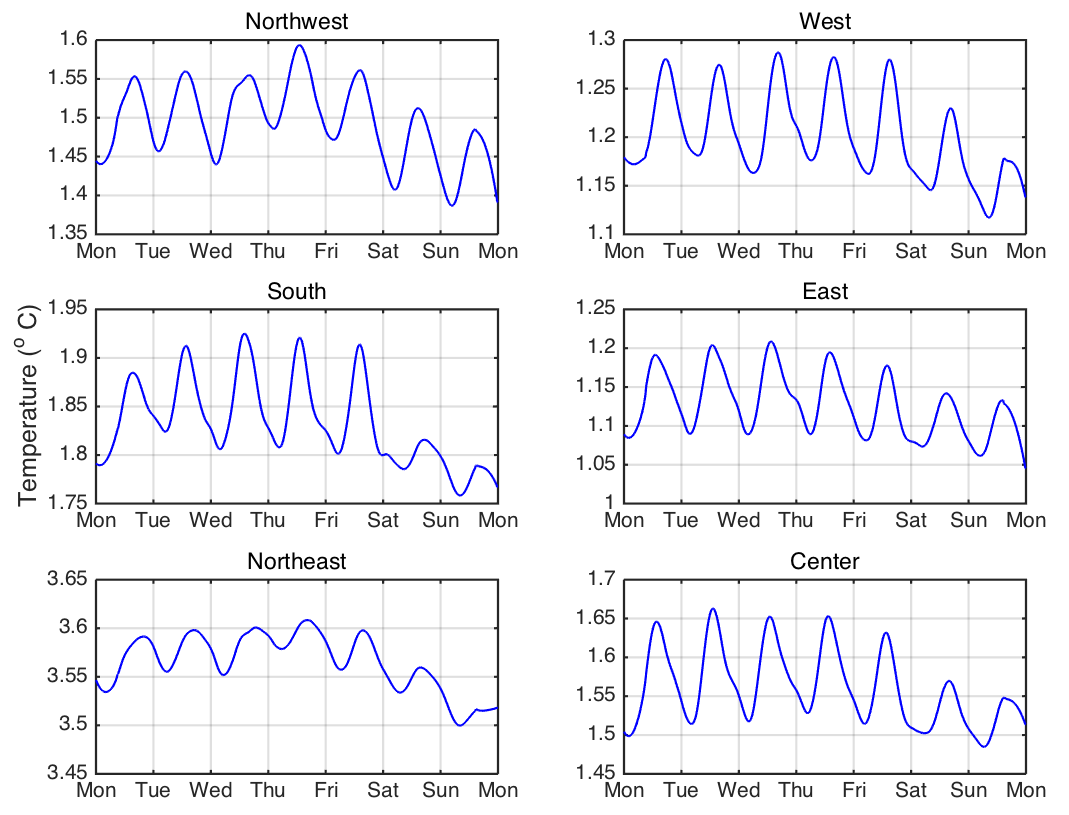
\includegraphics[scale=0.40]{chapters/building_exp/figures/data_indiv_qig_fall.png}
%\vspace*{-0.2cm}
\caption{Estimated internal gains by zone.}
\label{fig:qig}
\vspace*{-0.25cm}
\end{figure}

\begin{figure}[t]
\centering
%\vspace*{-0.4cm}
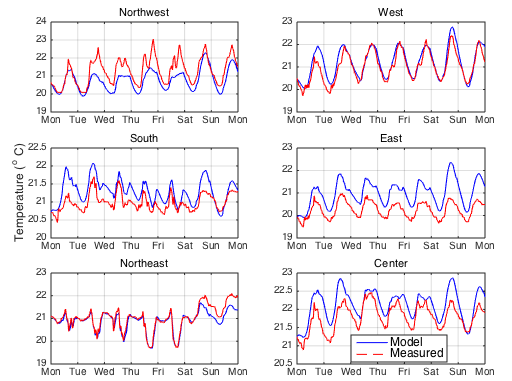
\includegraphics[scale=0.40]{chapters/building_exp/figures/open_loop_traj_spring.png}
%\vspace*{-0.2cm}
\caption{Open-loop temperature prediction by zone.}
\label{fig:building_prediction}
\vspace*{-0.45cm}
\end{figure}


%%%%%%%%%%%%%%%%%%%%%%%%%%%%%%%%%%%%%%%%%%%%%%
%%%%%%%%%%%%%%%%%%%%%%%%%%%%%%%%%%%%%%%%%%%%%%

\subsubsection{Results}

Figure \ref{fig:qig} shows the estimated internal gains $\hat{q}$ for the six zones. It can be seen that the different zones exhibit different magnitudes of internal gains, with average values of the internal gains ranging between 1.0$^{\circ}$C and 3.6$^{\circ}$C for different zones. 
Furthermore, the internal gains exhibit a daily trend with local peaks around the late afternoon and local minima at night. Moreover, the amplitudes of the internal gains are considerably smaller during the weekends, suggesting a lighter occupancy.
%daily peaks of the internal gains profiles can be recognized, with a slight decrease in magnitude on weekend days. 
The average root-mean-square (RMS) prediction errors by zone are reported in Table \ref{tab:data_RMS_zones}.	
Figure \ref{fig:building_prediction} shows 7-day open-loop predictions of the temperature of a randomly selected holdout test week.

\begin{table}[]
	\centering
	\caption{RMS prediction error by zone for building model in $^{\circ}$C.}
	\label{tab:data_RMS_zones}
	\begin{tabular}{*6c | c}
	\toprule
	Northwest & West & South & East & Northeast & Center & Mean \\ \hline
	%Fall & 0.98 & 0.61 & 0.28 & 0.42 & 0.28 & 0.36 & 0.488\\
	%Winter & 1.41 & 0.34 & 0.29 & 0.26 & 0.25 & 0.21 & 0.460\\
	0.56 & 0.25 & 0.31 & 0.71 & 0.17 & 0.34 & 0.390\\
	\bottomrule
	\end{tabular}
\end{table}

%\begin{table*}[]
%	\centering
%	\caption{Backward Reachable Set Decomposition}
%	\label{table:summary_BRS}
%  \footnotesize{
%	\begin{tabular}{|l|l|l|l|l|}
%		\hline
%		\textbf{Section}            & \multicolumn{2}{c|}{\textbf{\ref{sec:sc}}}   & \multicolumn{2}{c|}{\textbf{\ref{sec:decoupled}}} \\ \hline
%		\textbf{Shared Controls}    & \multicolumn{2}{c|}{\textbf{Yes}}  & \multicolumn{2}{c|}{\textbf{No}} \\ \hline
%		\textbf{Shared Disturbance} & \multicolumn{2}{c|}{\textbf{No}}   & \multicolumn{2}{c|}{\textbf{No}} \\ \hline
%		\textbf{Target}             & \textbf{Intersection} & \textbf{Union}      & \textbf{Intersection} & \textbf{Union} \\ \hline
%		Recover Max. BRS?  & No           & Yes, exact & Yes, exact   & Yes, exact \\ \hline
%		Recover Min. BRS?  & Yes, exact   & No         & Yes, exact   & Yes, exact \\ \hline
%		Locations \& Equation(s)        & Thm \ref{thm:sc_reach_in}, (\ref{eq:targetset_in})  & Thm \ref{thm:sc_reach_un}, (\ref{eq:targetset_un})         & \begin{tabular}[c]{@{}l@{}}Prop \ref{prop:decoupled_reach_in}, (\ref{eq:targetset_in_decoupled})\\ Thm \ref{thm:sc_reach_in}, (\ref{eq:targetset_in})\end{tabular} & \begin{tabular}[c]{@{}l@{}}Thm \ref{thm:sc_reach_un}, (\ref{eq:targetset_un})\\ Prop \ref{prop:decoupled_reach_un}, (\ref{eq:targetset_un_decoupled})\end{tabular} \\ \hline
%	\end{tabular}
%	\begin{tabular}{|l|l|l|l|l|}
%  \hline
%  \textbf{Section}            & \multicolumn{2}{c|}{\textbf{\ref{sec:sc_dstb}}} & \multicolumn{2}{c|}{\textbf{\ref{sec:decoupled_dstb}}} \\ \hline
%  \textbf{Shared Controls}    & \multicolumn{2}{c|}{\textbf{Yes}}    & \multicolumn{2}{c|}{\textbf{No}}     \\ \hline
%  \textbf{Shared Disturbance} & \multicolumn{2}{c|}{\textbf{Yes}}    & \multicolumn{2}{c|}{\textbf{Yes}}    \\ \hline
%  \textbf{Target}            & \textbf{Intersection}  & \textbf{Union}       & \textbf{Intersection}  & \textbf{Union}       \\ \hline
%  Recover Max. BRS? & No            & Yes, consrv & Yes, consrv   & Yes, consrv          \\ \hline
%  Recover Min. BRS? & Yes, consrv   & No          & Yes, consrv            & Yes, consrv \\ \hline
%  Locations \& Equation(s)       & Cor \ref{cor:minBRS_Intersection_SCS_Disturbance}, (\ref{eq:minBRS_intersection_disturbance}) & Cor \ref{cor:maxBRS_Union_SCS_Disturbance},  (\ref{eq:maxBRS_union_disturbance}) & Cor \ref{cor:targetset_in_decoupled_with_dstb}, (\ref{eq:targetset_in_decoupled_with_dstb}) & Cor \ref{cor:targetset_un_decoupled_with_dstb}, (\ref{eq:targetset_un_decoupled_with_dstb})           \\ \hline
%\end{tabular}
%}
%	\bigskip
%	\begin{flushleft}
%	 Summary of possible decompositions of the BRS, whether they are possible, and if so whether they are exact or conservative. Exact means that no additional approximation errors are introduced. Note that in the cases marked ``no" for shared control (or shared disturbance), the results hold for both decoupled control (or disturbance) and for no control (or disturbance). All cases shown are for scenarios with shared states, with the shared states being $\spart_c$ in \eqref{eq:scdyn}; in the case that there are no shared states this becomes a straightforward decoupled system.
%	\end{flushleft}
%\end{table*}

%%%%%%%%%%%%%%%%%%%%%%%%%%%%%%%%%%%%%%%%%%%%%%
%%%%%%%%%%%%%%%%%%%%%%%%%%%%%%%%%%%%%%%%%%%%%%
%%%%%%%%%%%%%%%%%%%%%%%%%%%%%%%%%%%%%%%%%%%%%%
%%%%%%%%%%%%%%%%%%%%%%%%%%%%%%%%%%%%%%%%%%%%%%


\subsubsection{Fan Model}

A fan model is identified from 6 weeks of one-minute resolution data for the supply fans collected from sMAP.
The fan laws state that the airflow rate through the fan is proportional to the fan speed, and the fan power is a cubic function of its speed \cite{Hvac_book}. 
Figure \ref{fig:fan_model} confirms the linear relationship between the airflow rate and the fan speed. 
The same figure also shows that there is little difference between the best fit quadratic and cubic curves for the relationship between the fan power and fan speed, suggesting that for the range of fan speeds plotted, a quadratic function can describe this relationship without significant loss of accuracy compared to a cubic function. %for fan speed between 28\% and 90\% of its maximum.
%The best fit quadratic and cubic curves for the relationship between the fan power and fan speed are also shown in the figure and they suggest that a quadratic function is able to describe this relationship without significant loss of accuracy compared to a cubic function. 
Since a quadratic function would simplify the subsequent controller design problem, it is adopted in this work. 
%Assume both supply fans are controlled to the same speed. 
%Let $N$ denote the fan speed of both fans, $u$ the total airflow rate through the fans and $P$ the total power consumption of the fans, then the fan model is defined as follows:
Let $N$ denote the fans' speed, $u$ the total airflow through the fans and $P$ the total fan power consumption, then the fan model is given as follows:
\begin{equation}\label{eq:fan_model}
\begin{aligned}
N & = f(u) = a_1 u + a_2\\
P & = g(N) = b_1 N^2 + b_2 N + b_3\\
P & = h(u) = c_1 u^2 + c_2 u + c_3.\\
\end{aligned}
\end{equation} 

\begin{figure}[t]
\centering
%\vspace*{-0.4cm}
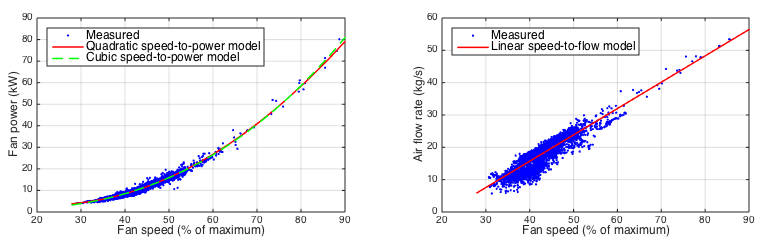
\includegraphics[scale=0.33]{chapters/building_exp/figures/fan_model.png}
\caption{Fan measurements and identified models for fan power and air flow as functions of fan speed.}
\label{fig:fan_model}
\vspace*{-0.15cm}
\end{figure}








